\section{}
The gauge pressure of the air in the tank shown in the figure below is
measured to be 50 kPa. Determine the differential height h of the mercury column.

\begin{figure}[h]
    \centering
    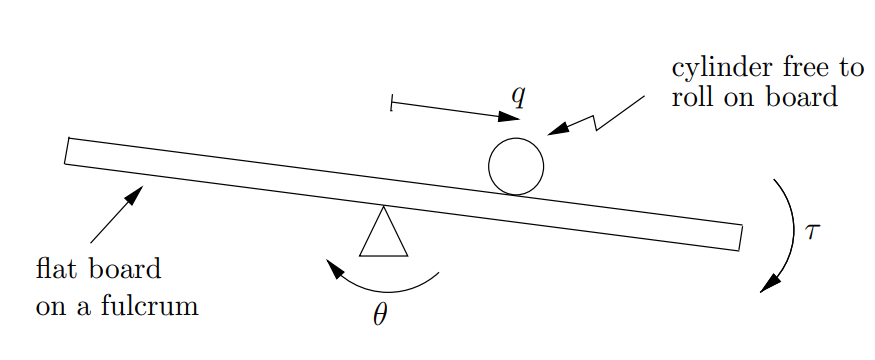
\includegraphics[width=0.5\textwidth]{Questions/Figures/Q4ProblemDiagram.png}
    \caption{Monometer with multiple fluids}
    \label{fig:Q4 System}
\end{figure}

The pressure balance for the system is given by:
\begin{align}
    P_{\text{air}} + P_{\text{w}} - P_{\text{Hg}} - P_{\text{oil}} = P_{\text{atm}} \nonumber
\end{align}

Isolating for $P_{gauge}$:
\begin{align}
    %P_{gauge} = P_{air}-P_{atm} = P_{Hg} + P_{oil} - P_{w} \nonumber
    P_{\text{gauge}} &= P_{\text{air}} - P_{\text{atm}} \nonumber \\
    &= P_{\text{Hg}} + P_{\text{oil}} - P_{\text{w}} \nonumber \\
    &= \rho_{\text{Hg}} g h_1 + \rho_{\text{oil}} g h_{2} - \rho_{\text{w}} g h_3 \nonumber \\
    % isolate for h_1
    \implies h_1 &= \frac{P_{\text{gauge}} + \rho_{\text{w}} g h_3 - \rho_{\text{oil}} g h_2}{\rho_{\text{Hg}} g} \label{eq:Q4hHg}
\end{align}

Finding densities
\begin{align*}
    \rho_w &= \qty{1000}{\kilogram\per\meter\cubed} \\
    \rho_{\text{Hg}} &= \qty{13600}{\kilogram\per\meter\cubed} \\
    \rho_{\text{oil}} &= \qty{720}{\kilogram\per\meter\cubed} 
\end{align*}

Substituting into (\ref{eq:Q4hHg})
\begin{align}
    % dont use qty
    h_1 &= \frac{50000 + 1000 \times 9.81 \times 0.3 - 720 \times 9.81 \times 0.75}{13600 \times 9.81} \nonumber \\
    &= \boxed{\qty{0.357}{\meter}} \nonumber
\end{align}